\documentclass{aiaa-tc}

%\usepackage[margin=1.0in]{geometry}
\usepackage{fullpage}
\usepackage{graphicx}
\usepackage{bm} %required for bold in math mode for greek symbols
\usepackage{amsmath} %for bmatrix
\usepackage{amsfonts} %for math script font
\usepackage{url} %for website citations

\usepackage[space]{grffile} %for filepaths with spaces

\setcounter{MaxMatrixCols}{15} % for bigger bmatrices

%define degree symbol:
\newcommand{\degree}{\ensuremath{^\circ}}

\newcommand{\fr}[1]{$#1^+$} %command to write a reference frame
\newcommand{\br}[2]{[#1]_{#2}} %bracket operator with subscript
\newcommand{\tvect}[3]{\begin{bmatrix}#1\\#2\\#3\end{bmatrix}}% 3 x 1 vector
\newcommand{\tvecth}[3]{\begin{bmatrix}#1&#2&#3\end{bmatrix}}% 1 x 3 vector
\newcommand{\B}[1]{\textbf{#1}} %bold for regular vectors
\newcommand{\U}[1]{\hat{\textbf{#1}}} %hats and bold for unit vectors
\newcommand{\BG}[1]{{\bm #1}}           % for vectors using greek letters
\newcommand{\ddt}[1]{\frac{d#1}{dt}} %for time derivatives
\newcommand{\ddarg}[2]{\frac{d#1}{d#2}} % for general derivatives
\newcommand{\pparg}[2]{\frac{\partial#1}{\partial#2}} % for general derivatives
\newcommand{\kron}{\otimes} %redefines \kron to produce kronecker product symbol, for convenience

\title{Summary of 2D cooperative estimation \\ \large{Feature bearing measurements only, known features}}
\author{Tim Woodbury}

\let\endtitlepage\relax %surpress line break after title page

\begin{document}

\maketitle

\section{Theoretical background}

We consider the problem of two agents that follow open-loop velocity trajectories. These agents move in a two-dimensional space and take bearing measurements of features that have known positions. The agents have inertial measurement units (IMUs) that record accelerations and angular velocity with Gaussian white noise. The agents also make relative range and bearing measurements of one another. To utilize these interagent measurements, the agents also communicate their feature bearing measurements and their measurement of the agent's bearing to one another.

In progressing, the notation $\B{r}_{ji}$ is used to delineate the vector from entity $i$ to $j$; letting $\B{r}_j$ and $\B{r}_i$ be the inertial position vectors to $j$ and $i$ respectively, $\B{r}_{ji} = \B{r}_j - \B{r}_i$. Since feature locations in an inertial reference frame are known, each agent estimates its own inertial position vector $\B{r}_i$, coordinatized in a body-fixed reference frame, and its inertial velocity $\B{v}_i$ and heading $\psi$, also expressed in the body frame. 

\subsection{Formulation}

For faster batch simulation, the problem has been addressed with a fully discrete Extended Kalman Filter using a first-order approximation to the derivatives. This has been compared against a continuous-discrete EKF and found not to differ substantially.

\begin{align}
\B{x}_{k+1} = T_s\dot{\B{x}}_k +\B{x}_k + G_k \B{w}_k, \B{w}_k \sim N(0,\B{Q}_k)  \\
 = \B{f}(\B{x},\B{u}) + G_k \B{w}_k\\
\tilde{\B{y}_k} = \B{h}(\B{x}_k) + \B{v}_k, \ \B{v}_k \ \sim N(0,\B{R}_k)\\
P_k \equiv E\{ \B{x}_k^T \B{x}_k \} \\
F(\hat{\B{x}}_k) \equiv \ddarg{\B{f}}{\B{x}} |_{\hat{\B{x}}_k^+} \\
H_k (\hat{\B{x}}_k^-) \equiv \ddarg{\B{h}}{\B{x}} |_{\hat{\B{x}}_k^-} \\
K_k \equiv P_k^-H_k^T(H_kP_k^-H_k^T + R_k)^{-1}\\
\hat{\B{x}}_k^+ = \hat{\B{x}}_k^- + K_k(\tilde{\B{y}} - \B{h}(\hat{\B{x}},\B{u}))\\
P_k^+ = (\B{I} - K_k H_k)P_k^-\\
\hat{\B{x}}_{k+1}^+ = \B{f}(\hat{\B{x}}_k^+,\B{u}) \\
P_{k+1}^+ = F_kP_k^+F_k^T + G_kQ_kG_k^T
\end{align}

\subsection{Propagation equations}

In vector form, the governing dynamic equations for agent $i$ are:

\begin{align}
\hat{\B{x}} = \begin{bmatrix}
\B{r}_i \\
\B{v}_i \\
\psi
\end{bmatrix}\\
{}^b \ddt{\B{r}_i} = \dot{\B{r}}_{i} = \B{v}_i - \BG{\omega}_i \times \B{r}_i \\
\br{\B{r}_i}{b} = \begin{bmatrix}
r_{i1}\\
r_{i2}
\end{bmatrix} \label{eq:gov_r} \\
{}^n \ddt{\B{r}_i} \equiv \B{v}_i \\
\br{\dot{\B{r}}_i}{b} = \begin{bmatrix}
v_1 + \omega_i r_{i2} \\
v_2 - \omega_i r_{i1}
\end{bmatrix} \\
\ddt{\psi} = \omega_i \label{eq:gov_psi} \\
{}^n \ddt{\B{v}_i} \equiv \B{a}_i \\
\br{\B{a}_i}{b} = \begin{bmatrix}
a_1 \\a_2
\end{bmatrix} \\
\br{\dot{\B{v}}_i}{b} = \begin{bmatrix}
a_1 + \omega_i v_{2} \\
a_2 - \omega_i v_1
\end{bmatrix} \label{eq:gov_v}
\end{align}

Eqs. \ref{eq:gov_r},\ref{eq:gov_psi}, and \ref{eq:gov_v} are the governing equations of motion for agent $i$. These equations are incorporated in the Extended Kalman Filter as propagation equations, treating the IMU measurements as inputs to the governing equations. Process noise becomes associated with these equations through propagation of the sensor uncertainty. Letting $\tilde{x}$ represent a measurement of random variable $x$, the process noise influence terms can be arrived at by simple substitution:

\begin{align}
\tilde{\B{a}}_i = \B{a}_i + \B{v}_a \\
\tilde{\omega}_i = \omega_i + v_\omega \\
\br{\dot{\B{v}}_i}{b} = \begin{bmatrix}
\tilde{a}_1 - v_{a1} + \tilde{\omega}_i v_{2} -  v_\omega v_2\\
\tilde{a}_2 - v_{a2} - \tilde{\omega}_i v_1 + v_\omega v_1
\end{bmatrix} \\
\dot{\psi} = \omega_i = \tilde{\omega}_i - v_\omega \\
\begin{bmatrix}
\dot{v}_1 \\ \dot{v}_2 \\ \dot{\psi}
\end{bmatrix}= \begin{bmatrix}
0 & \tilde{\omega} \\ -\tilde{\omega} & 0 \\ 0 & 0
\end{bmatrix} \begin{bmatrix}
v_1\\ v_2
\end{bmatrix} + \begin{bmatrix}
\tilde{a}_1 \\ \tilde{a}_2 \\ \tilde{\omega}_i
\end{bmatrix} + \begin{bmatrix}
-1 & 0 & -v_2 \\
0 & -1 & v_1 \\
0 & 0 & -1
\end{bmatrix} \begin{bmatrix}
v_{a1} \\ v_{a2} \\ v_\omega
\end{bmatrix} \label{eq:prop_eq} \\
\end{align}

Eqs. \ref{eq:gov_r}-\ref{eq:prop_eq} contains nonzero elements of the process noise influence matrix $G_k$. The gradient of the propagation equation with respect to the estimated states can be written as:

\begin{equation}
\ddarg{\B{f}(\B{x},\B{u})}{\B{x}} = F_k = \B{I}_{5\times 5} + T_s\begin{bmatrix}
\begin{bmatrix}
0 & \tilde{\omega} \\ -\tilde{\omega} & 0
\end{bmatrix} & \B{I}_{2\times 2} & \B{0}_{2\times 1} \\
\B{0}_{2\times 2} & \begin{bmatrix}
0 & \tilde{\omega} \\ -\tilde{\omega} & 0
\end{bmatrix} & \B{0}_{2\times 1} \\
& \B{0}_{1 \times 5} &
\end{bmatrix}
\end{equation}

The process noise covariance $Q_k$ is simply the covariance matrix associated with the IMU, $R_{IMU}$. The continuous-time Kalman propagation equations can now be written:

\begin{align}
G_k \equiv T_s\begin{bmatrix}
0 & 0 & -r_2 \\0 & 0 & r_1\\
-1 & 0 & -v_2 \\
0 & -1 & v_1 \\
0 & 0 & -1
\end{bmatrix} \\
\hat{\B{x}}_{k+1}^+ = \B{f}(\hat{\B{x}}_k^+,\B{u}) \label{eq:gov_ddt_est}\\
P^{+}_{k+1} = F_kP_k^{-}F_k^T + G_k R_{IMU} G_k^T \label{eq:gov_ddt_cov}
\end{align}

Eqs. \ref{eq:gov_ddt_est} and \ref{eq:gov_ddt_cov} are the governing equations for the estimated states $\hat{\B{x}}$ and associated a priori error covariance $P^-$.

\subsection{Measurement model}

\begin{figure}[tb!]
\centering
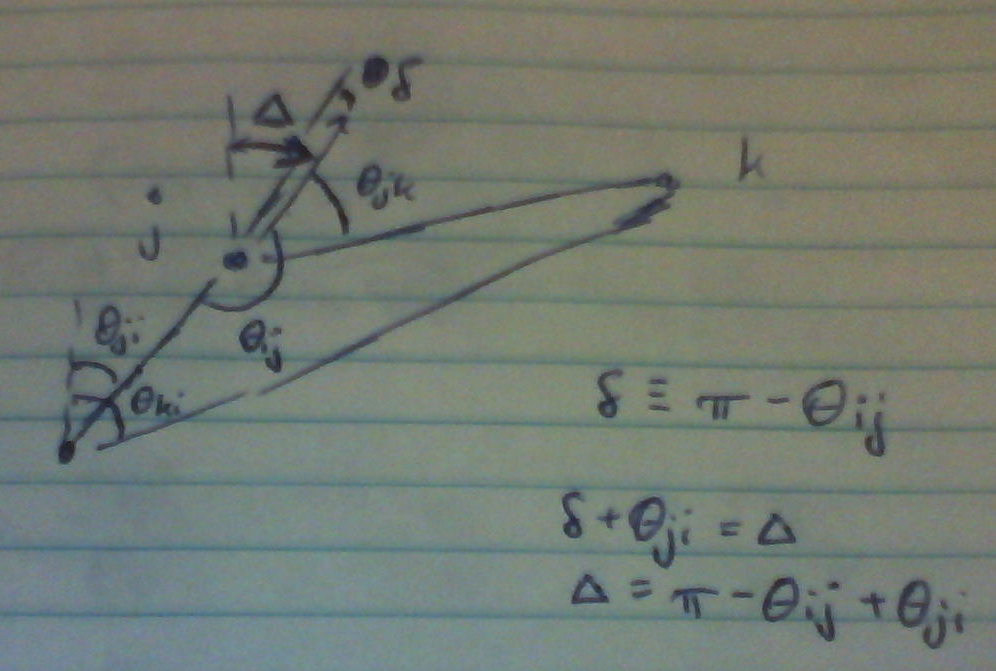
\includegraphics[width=0.8\textwidth]{geometry.png}
\caption{Problem geometry.}
\label{fig:geometry}
\end{figure}

Define the vector from agent $i$ to agent $j$ as $\B{r}_{ji}$. Bearing measurements are defined as the arctangent of the ratio of the two-axis component of a vector from an agent to a target to the one-axis component, when the vector is coordinatized in the agent's body reference frame. For planar motion, any bearing measurement made in one reference frame can be compared against a value in a different frame by adding the relative heading between the two reference frames. The objective of shared measurements is to take measurements of feature $k$ made by agent $j$ and compare them against the values agent $i$ expects to see, given $i$'s position relative to the feature and relative to agent $j$. In the most general sense, the vectors between the two agents and the feature are governed by:

\begin{equation}
\B{r}_{kj} = \B{r}_{ki} - \B{r}_{ji}
\end{equation}

In this scenario, $\B{r}_{kj}$ is not fully observed. The bearing measurement made by $j$ can be defined as follows:

\begin{align}
\B{r}_{kj} = \begin{bmatrix}
r_{kj1} \\
r_{kj2}
\end{bmatrix}\\
\tan{\theta_{kj}} = \frac{r_{kj2}}{r_{kj1}}
\end{align}

In general, however, $\B{r}_{kj}$ is estimated only by $j$, and is not known by $i$. $i$ does estimate $\B{r}_{ki}$ and measures $\B{r}_{ji}$ in its own body frame. Define the angle $\Delta$ as the rotation angle from agent $i$'s frame to agent $j$'s. Call $\theta_{kj}^{'}$ the $i$ frame expectation of $\theta_{kj}$, and note that $\theta_{kj}^{'} = \theta_{kj} + \Delta$.

\begin{align}
\B{r}_{ki} = \begin{bmatrix}
r_{ki1} \\r_{ki2}
\end{bmatrix}\\
\theta_{kj} + \Delta = \arctan{ \frac{r_{ki2} - \rho_{ji}\sin{\theta_{ji}}}{r_{ki1} - \rho_{ji}\cos{\theta_{ji}}} }\\
\Phi = \arctan{ \frac{\hat{r}_{ki2} - \tilde{\rho}_{ji}\sin{\tilde{\theta}_{ji}}}{\hat{r}_{ki1} - \tilde{\rho}_{ji}\cos{\tilde{\theta}_{ji}}} } - \tilde{\theta}_{kj} - \tilde{\Delta} \label{eq:phidef}
\end{align}

$\Delta$, for the case of planar motion, is a straightforward function of the inter-agent relative bearing measurements made by agents $i$ and $j$. $\theta_{ij}$ is agent $j$'s measurement of $i$, and $\theta_{ji}$ is $i$'s measurement of $j$:

\begin{equation}
\Delta = \pi - \theta_{ij} + \theta_{ji}
\end{equation}

Eq. \ref{eq:phidef} is a nonlinear function of both estimated values and measurements, and the estimates cannot in general be isolated. For implementation, this equation is treated as a constraint whose expectation is always zero. As in the scenario when feature range and bearing are measured, statistical linearization is used to compute the covariance matrix associated with the constraint equation. As in the previous scenario, the parameter $\alpha$ is set to 1 for linearization. (Note: As a check, covariances obtained from linearization were compared against results achieved using the constraint Jacobian and found to be similar.)

\section{Simulation}

Simulation is conducted to determine the effectiveness of sharing measurements, and also to examine the loss in accuracy compared to the case where feature range is measured. First, performance with and without feature range measurements is compared, for both cooperating and individual agents. Iteratively larger variance is placed on feature range measurements to determine approximately when shared measurements become comparable to feature range in terms of localization accuracy. Second, simulations are conducted with measurements being shared at reduced rates. Third, simulations are conducted with a small number of features in the workspace, to highlight the effect of shared measurements. Finally, simulations with relatively large numbers of features present are executed.

In each Monte Carlo simulation, the same open-loop agent trajectories and feature locations are used with sensor noise that is generated at runtime. Features are randomly placed within 20 meters of the inertial coordinate system origin, with uniformly distributed radius and bearing angle in polar coordinates. Agents are initialized with a normally distributed initial radius having standard deviation 5 m, and uniformly distributed polar angle. Agents follow trajectories for radial position $r(t)$, polar coordinate $\theta(t)$, and heading angle $\psi(t)$ according to:

\begin{align}
r(t) = r(0) + a\sin{wt}
\label{eq:r_t} \\
\theta(t) = \theta(0) + Wt \\
\psi(t) = \psi(0) + \omega t \label{eq:psi_t}
\\
W = \pi/20 \\
w = 2.2W\\
\omega = -\mathrm{sign}(\psi(0)) 0.4
\end{align}

Agent velocities are specified to satisfy Eqs. \ref{eq:r_t}-\ref{eq:psi_t}. Agent truth histories are generated up to the acceleration level for translation and to the velocity level for rotation. In addition to the interagent range and bearing sensors and the feature bearing sensors, agents possess inertial measurement units that measure translational acceleration and angular velocity. Sensors are assumed to have no bias with normally distributed random additive errors. All bearing measurements have variance $0.01$ and interagent range measurements have variance $1$, unless specified otherwise. Interagent sensors are assumed to have a 360\degree \ field of view and infinite range sensitivity; feature detection sensors are assumed to have 30\degree \ half-angle fields of view, and sensitivity at ranges between 1 and 10 meters, unless specified otherwise.

For the simulations presented here, agent initial conditions are set to the truth values. The covariance matrix is initialized as a fully populated matrix of 0.001, plus diagonal elements of $\begin{bmatrix}1.2 & 1.2 & 0.64 & 0.64 & 0.03\end{bmatrix}$. Performance was not, in general, found to be highly dependent on the covariance initialization.

\subsection{Comparison against feature range and bearing measurements}\label{sec:subc1}

In this section, the effect of providing feature range measurements is contrasted with cooperative bearing-only measurements. Tables \ref{tab:feature_r&b}--\ref{tab:feature_bonly} show standard errors $S$ and mean squared errors $MSE$ for each estimated state in 100 Monte Carlo simulations. All bearing measurements have variance $.01$ and all range measurements have variance $1$ unless stated otherwise. 15 features with known inertial frame $X-Y$ positions are present. Tables \ref{tab:feature_r&b}-\ref{tab:feature_r&b_10} are for the case where feature range and bearing are both measured. Only individual results are presented for this case; cooperation improves accuracy but is not of direct interest in this section. 

Table \ref{tab:feature_bonly} shows results when feature bearings only are measured. Sharing measurements substantially reduces errors in position and heading. In considering the effect of adding feature range detection versus adding shared measurements, it appears that feature range measurements are more useful at a variance level of 1, but less useful at a variance of 10 compared to shared measurements. This suggests that if the quality of feature range measurements is low, this cooperative estimation scheme may be particularly practical.

\begin{table}[b!]
\scriptsize
\centering
\begin{tabular}{c|c|c|c|c|c|c|c|c|c|c|c|}
Case & Agent & $S(\epsilon_{rix})$ & $S(\epsilon_{riy})$ & $S(\epsilon_{u})$ & $S(\epsilon_{v})$ & $S(\epsilon_{\psi})$ & $MSE(r_{ix})$ & $MSE(r_{iy})$ & $MSE(u)$ & $MSE(v)$ & $MSE(\psi)$ \\
Individual & 1& 0.749& 0.649& 0.199& 0.205& 0.0354& 0.561& 0.424& 0.0401& 0.042& 0.00156 \\
Individual & 2& 0.528& 0.506& 0.171& 0.18& 0.0283& 0.279& 0.256& 0.0295& 0.0324& 0.000803
\end{tabular}
\caption{Monte Carlo estimation errors with feature range and bearing measurements. Feature range variance is 1.}
\label{tab:feature_r&b}
\end{table}

\begin{table}[b!]
\scriptsize
\centering
\begin{tabular}{c|c|c|c|c|c|c|c|c|c|c|c|}
Case & Agent & $S(\epsilon_{rix})$ & $S(\epsilon_{riy})$ & $S(\epsilon_{u})$ & $S(\epsilon_{v})$ & $S(\epsilon_{\psi})$ & $MSE(r_{ix})$ & $MSE(r_{iy})$ & $MSE(u)$ & $MSE(v)$ & $MSE(\psi)$ \\
Individual & 1& 1.33& 0.973& 0.259& 0.239& 0.0534& 1.8& 1.01& 0.0715& 0.0571& 0.00317 \\
Individual & 2& 0.808& 0.653& 0.199& 0.198& 0.038& 0.656& 0.429& 0.0398& 0.0392& 0.00145 
\end{tabular}
\caption{Monte Carlo estimation errors with feature range and bearing measurements. Feature range variance is 10.}
\label{tab:feature_r&b_10}
\end{table}

\begin{table}[tb!]
\scriptsize
\centering
\begin{tabular}{c|c|c|c|c|c|c|c|c|c|c|c|}
Case & Agent & $S(\epsilon_{rix})$ & $S(\epsilon_{riy})$ & $S(\epsilon_{u})$ & $S(\epsilon_{v})$ & $S(\epsilon_{\psi})$ & $MSE(r_{ix})$ & $MSE(r_{iy})$ & $MSE(u)$ & $MSE(v)$ & $MSE(\psi)$ \\
Individual & 1& 1.63& 1.37& 0.257& 0.239& 0.0531& 2.79& 2.09& 0.0786& 0.0582& 0.00315 \\
Cooperative & 1& 0.98& 0.654& 0.219& 0.202& 0.0334& 1.1& 0.445& 0.0565& 0.0409& 0.00118 \\
Individual & 2& 0.975& 0.684& 0.214& 0.189& 0.0283& 0.969& 0.535& 0.0501& 0.0366& 0.000799 \\
Cooperative & 2& 0.713& 0.668& 0.213& 0.21& 0.0307& 0.52& 0.479& 0.0483& 0.0449& 0.000943 
\end{tabular}
\caption{Monte Carlo estimation errors with only feature bearing measurements.}
\label{tab:feature_bonly}
\end{table}

\subsection{Reduced sharing rate}

In the other simulations conducted, measurements are shared at the same rate they are taken, 10 Hz. In this section the effect of reduced sharing rates is considered. 1000 Monte Carlo simulations are conducted in each run, in an effort to ensure that statistically significant results are obtained. Additionally, initial conditions have normally distributed errors with standard deviation of 1 m for position, 0.25 m/s for speed, and 0.03 rad for heading.

Results are presented in Tables \ref{tab:K_5}-\ref{tab:K_100} for sharing rates of 2, 1, 0.4, and 0.1 Hz. Individual agent results are also presented, as a baseline for comparison. In general, cooperation appears to have some benefit at all rates, although the effect is minimal at 0.1 and 0.4 Hz and may not justify the added computational and communications overhead. However, use of this estimation scheme can probably be justified at 1 Hz for many setups. This approximately 10\% sharing rate ``limit'' is consistent with previously obtained results with feature range and bearing measurements.

\begin{table}[b!]
\scriptsize
\centering
\begin{tabular}{c|c|c|c|c|c|c|c|c|c|c|c|}
Case & Agent & $S(\epsilon_{rix})$ & $S(\epsilon_{riy})$ & $S(\epsilon_{u})$ & $S(\epsilon_{v})$ & $S(\epsilon_{\psi})$ & $MSE(r_{ix})$ & $MSE(r_{iy})$ & $MSE(u)$ & $MSE(v)$ & $MSE(\psi)$ \\
Individual & 1& 1.37& 1.09& 0.258& 0.234& 0.0568& 2.05& 1.41& 0.0801& 0.0559& 0.00362 \\
Cooperative & 1& 1.08& 0.801& 0.233& 0.216& 0.0463& 1.3& 0.726& 0.0639& 0.0468& 0.00243 \\
Individual & 2& 1.04& 0.731& 0.223& 0.201& 0.032& 1.11& 0.613& 0.0542& 0.0415& 0.00103 \\
Cooperative & 2& 0.798& 0.645& 0.209& 0.197& 0.0291& 0.65& 0.472& 0.0471& 0.0395& 0.00085
\end{tabular}
\caption{Bearing-only Monte Carlo estimation errors with 2 Hz sharing frequency.}
\label{tab:K_5}
\end{table}

\begin{table}[b!]
\scriptsize
\centering
\begin{tabular}{c|c|c|c|c|c|c|c|c|c|c|c|}
Case & Agent & $S(\epsilon_{rix})$ & $S(\epsilon_{riy})$ & $S(\epsilon_{u})$ & $S(\epsilon_{v})$ & $S(\epsilon_{\psi})$ & $MSE(r_{ix})$ & $MSE(r_{iy})$ & $MSE(u)$ & $MSE(v)$ & $MSE(\psi)$ \\
Individual & 1& 1.5& 1.2& 0.26& 0.235& 0.0566& 2.4& 1.65& 0.0804& 0.0567& 0.00363 \\
Cooperative & 1& 1.24& 0.943& 0.247& 0.229& 0.0505& 1.68& 1.02& 0.0727& 0.0531& 0.00291 \\
Individual & 2& 1.05& 0.725& 0.223& 0.198& 0.0325& 1.11& 0.6& 0.0541& 0.0403& 0.00106 \\
Cooperative & 2& 0.851& 0.653& 0.21& 0.194& 0.0289& 0.739& 0.488& 0.0477& 0.0385& 0.000846
\end{tabular}
\caption{Bearing-only Monte Carlo estimation errors with 1 Hz sharing frequency.}
\label{tab:K_10}
\end{table}

\begin{table}[b!]
\scriptsize
\centering
\begin{tabular}{c|c|c|c|c|c|c|c|c|c|c|c|}
Case & Agent & $S(\epsilon_{rix})$ & $S(\epsilon_{riy})$ & $S(\epsilon_{u})$ & $S(\epsilon_{v})$ & $S(\epsilon_{\psi})$ & $MSE(r_{ix})$ & $MSE(r_{iy})$ & $MSE(u)$ & $MSE(v)$ & $MSE(\psi)$ \\
Individual & 1& 1.31& 1.02& 0.253& 0.233& 0.0567& 1.88& 1.23& 0.0768& 0.0553& 0.00362 \\
Cooperative & 1& 1.26& 0.959& 0.249& 0.227& 0.0533& 1.72& 1.08& 0.074& 0.0521& 0.00324 \\
Individual & 2& 1.02& 0.71& 0.22& 0.197& 0.0307& 1.05& 0.58& 0.0524& 0.0399& 0.000948 \\
Cooperative & 2& 0.925& 0.681& 0.217& 0.196& 0.0291& 0.875& 0.535& 0.0514& 0.0392& 0.000859
\end{tabular}
\caption{Bearing-only Monte Carlo estimation errors with 0.4 Hz sharing frequency.}
\label{tab:K_25}
\end{table}

\begin{table}[b!]
\scriptsize
\centering
\begin{tabular}{c|c|c|c|c|c|c|c|c|c|c|c|}
Case & Agent & $S(\epsilon_{rix})$ & $S(\epsilon_{riy})$ & $S(\epsilon_{u})$ & $S(\epsilon_{v})$ & $S(\epsilon_{\psi})$ & $MSE(r_{ix})$ & $MSE(r_{iy})$ & $MSE(u)$ & $MSE(v)$ & $MSE(\psi)$ \\
Individual & 1& 1.39& 1.1& 0.257& 0.234& 0.0571& 2.1& 1.41& 0.0791& 0.0562& 0.0037 \\
Cooperative & 1& 1.36& 1.07& 0.259& 0.234& 0.058& 2.01& 1.36& 0.0802& 0.0561& 0.00387 \\
Individual & 2& 1.03& 0.717& 0.221& 0.199& 0.031& 1.08& 0.591& 0.0528& 0.0405& 0.000965 \\
Cooperative & 2& 0.963& 0.691& 0.218& 0.195& 0.0304& 0.947& 0.549& 0.0516& 0.0392& 0.000933
\end{tabular}
\caption{Bearing-only Monte Carlo estimation errors with 0.1 Hz sharing frequency.}
\label{tab:K_100}
\end{table}

\pagebreak
\subsection{Small number of features}

In this section, bearing-only feature measurements with a reduced number of features in the workspace are considered. Agents follow the same open-loop trajectories as in Sec. \ref{sec:subc1} with measurement noises generated at runtime. Tables \ref{tab:M_5_features} and \ref{tab:M_4_features} show tabulated errors with five and four features, respectively. With five features, localization standard errors are on the order of meters in both the individual and cooperative cases (although mean squared errors are much higher in the former case!). Performance for the cooperative case is comparable to performance with fifteen features, has degraded much less than performance for the individual case.

In the case of four features, performance for both cases deteriorates significantly. Accuracy in the cooperative case is worse than in the individual case at five features, and mean squared errors in the individual cases at four features indicate that localization is effectively useless. Four features seems to represent the lower limit at which localization is possible for the trajectories and variance levels assumed.

\begin{table}[tb!]
\scriptsize
\centering
\begin{tabular}{c|c|c|c|c|c|c|c|c|c|c|c|}
Case & Agent & $S(\epsilon_{rix})$ & $S(\epsilon_{riy})$ & $S(\epsilon_{u})$ & $S(\epsilon_{v})$ & $S(\epsilon_{\psi})$ & $MSE(r_{ix})$ & $MSE(r_{iy})$ & $MSE(u)$ & $MSE(v)$ & $MSE(\psi)$ \\
Individual & 1& 3.54& 3.29& 0.383& 0.362& 0.103& 12.5& 11.2& 0.15& 0.135& 0.011 \\
Cooperative & 1& 1.67& 1.33& 0.274& 0.253& 0.0552& 2.82& 1.79& 0.0774& 0.0641& 0.00323 \\
Individual & 2& 2.52& 2.14& 0.289& 0.269& 0.067& 6.43& 4.74& 0.0862& 0.0744& 0.00452 \\
Cooperative & 2& 1.53& 1.41& 0.301& 0.298& 0.0393& 2.37& 2& 0.092& 0.0887& 0.0016
\end{tabular}
\caption{Bearing-only Monte Carlo estimation errors with 5 features in the workspace.}
\label{tab:M_5_features}
\end{table}

\begin{table}[tb!]
\scriptsize
\centering
\begin{tabular}{c|c|c|c|c|c|c|c|c|c|c|c|}
Case & Agent & $S(\epsilon_{rix})$ & $S(\epsilon_{riy})$ & $S(\epsilon_{u})$ & $S(\epsilon_{v})$ & $S(\epsilon_{\psi})$ & $MSE(r_{ix})$ & $MSE(r_{iy})$ & $MSE(u)$ & $MSE(v)$ & $MSE(\psi)$ \\
Individual & 1& 27.5& 27.2& 1.27& 1.34& 0.171& 759& 792& 1.62& 2& 0.0299 \\
Cooperative & 1& 7.2& 7.87& 0.575& 0.623& 0.101& 52.1& 63.1& 0.334& 0.396& 0.0108 \\
Individual & 2& 24.3& 24.6& 1.12& 1.12& 0.162& 591& 622& 1.27& 1.33& 0.0263 \\
Cooperative & 2& 5.07& 4.52& 0.466& 0.416& 0.0742& 26.9& 20.5& 0.234& 0.174& 0.00557
\end{tabular}
\caption{Bearing-only Monte Carlo estimation errors with 4 features in the workspace.}
\label{tab:M_4_features}
\end{table}

\subsection{Large number of features}

In this section, the number of features in the workspace is greatly increased. New open-loop agent trajectories are generated. The maximum feature detection range is reduced to 5 meters, to highlight the change in estimation accuracy as the number of features is increased. 25, 50, and 75 features are considered and results given in Tables \ref{tab:M_25_features}--\ref{tab:M_75_features}. As can be seen, there is a significant improvement in performance when the number of features increases from 25 to 50. However, between 50 and 75 features, the change in estimation error is generally in the second or lower significant figure(s), a clear indication of diminishing returns. Too, the performance of the individual and cooperative cases at 75 features is virutally indistinguishable, while there is still a noticeable difference in accuracy between the two cases at 50 features.

The actual limits of estimation performance are expected to be strongly dependent on the sensor accuracy and capabilities, the workspace itself, and the trajectories taken by the agents. 

\begin{table}[b!]
\scriptsize
\centering
\begin{tabular}{c|c|c|c|c|c|c|c|c|c|c|c|}
Case & Agent & $S(\epsilon_{rix})$ & $S(\epsilon_{riy})$ & $S(\epsilon_{u})$ & $S(\epsilon_{v})$ & $S(\epsilon_{\psi})$ & $MSE(r_{ix})$ & $MSE(r_{iy})$ & $MSE(u)$ & $MSE(v)$ & $MSE(\psi)$ \\
Individual & 1& 0.669& 0.509& 0.181& 0.165& 0.0324& 0.493& 0.311& 0.0389& 0.0272& 0.00111 \\
Cooperative & 1& 0.638& 0.496& 0.175& 0.158& 0.0266& 0.492& 0.351& 0.0421& 0.0253& 0.00102 \\
Individual & 2& 1.16& 0.943& 0.241& 0.219& 0.0517& 1.4& 1& 0.0659& 0.0485& 0.00419 \\
Cooperative & 2& 0.914& 0.672& 0.232& 0.202& 0.0301& 1.14& 0.508& 0.0729& 0.0411& 0.00125
\end{tabular}
\caption{Bearing-only Monte Carlo estimation errors with 25 features in the workspace.}
\label{tab:M_25_features}
\end{table}

\begin{table}[t!]
\scriptsize
\centering
\begin{tabular}{c|c|c|c|c|c|c|c|c|c|c|c|}
Case & Agent & $S(\epsilon_{rix})$ & $S(\epsilon_{riy})$ & $S(\epsilon_{u})$ & $S(\epsilon_{v})$ & $S(\epsilon_{\psi})$ & $MSE(r_{ix})$ & $MSE(r_{iy})$ & $MSE(u)$ & $MSE(v)$ & $MSE(\psi)$ \\
Individual & 1& 0.412& 0.305& 0.16& 0.138& 0.0221& 0.269& 0.113& 0.0348& 0.0196& 0.00052 \\
Cooperative & 1& 0.316& 0.292& 0.151& 0.131& 0.0207& 0.291& 0.13& 0.0408& 0.0177& 0.000647 \\
Individual & 2& 0.61& 0.472& 0.206& 0.185& 0.0289& 0.485& 0.252& 0.0521& 0.0343& 0.00149 \\
Cooperative & 2& 0.509& 0.317& 0.214& 0.181& 0.0252& 0.762& 0.122& 0.0745& 0.0365& 0.000696
\end{tabular}
\caption{Bearing-only Monte Carlo estimation errors with 50 features in the workspace.}
\label{tab:M_50_features}
\end{table}

\begin{table}[t!]
\scriptsize
\centering
\begin{tabular}{c|c|c|c|c|c|c|c|c|c|c|c|}
Case & Agent & $S(\epsilon_{rix})$ & $S(\epsilon_{riy})$ & $S(\epsilon_{u})$ & $S(\epsilon_{v})$ & $S(\epsilon_{\psi})$ & $MSE(r_{ix})$ & $MSE(r_{iy})$ & $MSE(u)$ & $MSE(v)$ & $MSE(\psi)$ \\
Individual & 1& 0.276& 0.167& 0.145& 0.12& 0.0198& 0.211& 0.0367& 0.0314& 0.0164& 0.000443 \\
Cooperative & 1& 0.269& 0.207& 0.147& 0.119& 0.0199& 0.301& 0.0698& 0.0422& 0.0165& 0.000618 \\
Individual & 2& 0.509& 0.414& 0.197& 0.179& 0.0264& 0.403& 0.206& 0.0513& 0.0323& 0.00103 \\
Cooperative & 2& 0.461& 0.295& 0.209& 0.177& 0.0253& 0.728& 0.104& 0.0717& 0.0376& 0.000642
\end{tabular}
\caption{Bearing-only Monte Carlo estimation errors with 75 features in the workspace.}
\label{tab:M_75_features}
\end{table}

\pagebreak
\section{Summary}

\begin{enumerate}
\item Measurement sharing for feature-based localization with only feature bearing measurements can substantially improve localization accuracy, depending on sensor characteristics and vehicle motion. When compared to localization using feature range measurements, cooperation may be more useful than feature range measurements, depending on the variance of the range measurements.
\item Measurement sharing at lower update rates improves estimation accuracy noticeably for rates an order of magnitude lower than the nominal sharing rate.
\item When the number of features in the workspace is low, performance degrades more slowly for the cooperative case than for the individual case.
\item When the number of features is quite large, there is a point of diminishing returns from cooperation. For the simulation considered, this point is somewhere between 50 and 75 features, which is considered to be a very large number for the workspace size considered.
\end{enumerate}

\bibliography{../../references}
\bibliographystyle{aiaa}

\end{document}
